\documentclass[tikz,border=3pt]{standalone}
\usepackage[utf8]{inputenc}
\usepackage[T1]{fontenc}
\usepackage{lmodern}
\renewcommand{\familydefault}{\sfdefault}
\usepackage{amsmath}
\usepackage{sansmath}\sansmath
\usepackage{pgfplots}\pgfplotsset{compat=1.18,/pgf/number format/use comma,/pgf/number format/1000 sep={.}}
\usetikzlibrary{arrows.meta,calc,positioning,decorations.pathmorphing,patterns}
% paleta del sitio
\definecolor{nar}{HTML}{E8680C}\definecolor{narc}{HTML}{FFB35C}\definecolor{hielo}{HTML}{FFF3E8}
\definecolor{tinta}{HTML}{1D1D1F}\definecolor{gris}{HTML}{6E6E73}\definecolor{lila}{HTML}{7C5CF0}
\definecolor{azul}{HTML}{2F6FD6}\definecolor{menta}{HTML}{17A673}\definecolor{coral}{HTML}{E8342A}
\pgfplotsset{base/.style={axis lines=left,grid=major,grid style={gris!20},tick label style={font=\small},label style={font=\small},axis line style={tinta!80}}}
\begin{document}
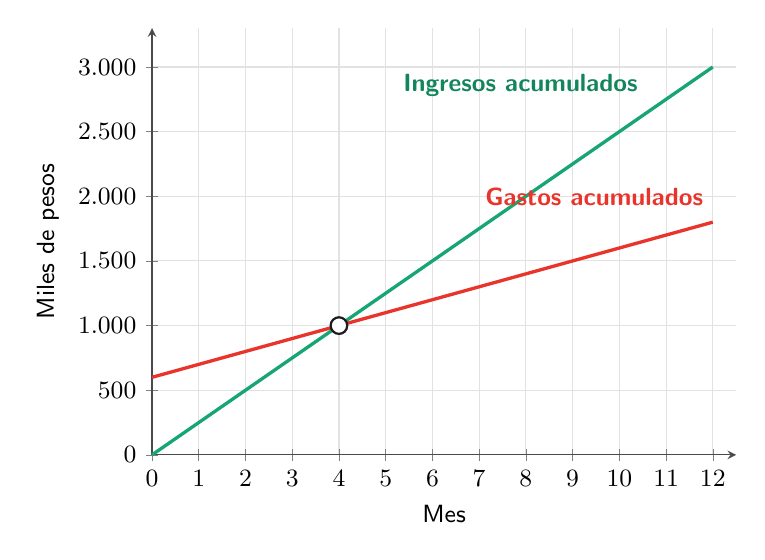
\begin{tikzpicture}
\begin{axis}[base,width=9cm,height=7cm,xmin=0,xmax=12.5,ymin=0,ymax=3300,xtick={0,...,12},ytick={0,500,...,3000},scaled y ticks=false,xlabel={Mes},ylabel={Miles de pesos},clip=false]
\addplot[coral,very thick,domain=0:12] {600+100*x};
\addplot[menta,very thick,domain=0:12] {250*x};
\addplot[only marks,mark=*,mark options={fill=white,draw=tinta,thick},mark size=3pt] coordinates {(4,1000)};
\node[coral,font=\small\bfseries,anchor=south east] at (axis cs:12,1850) {Gastos acumulados};
\node[menta!80!black,font=\small\bfseries,anchor=south east] at (axis cs:10.6,2700) {Ingresos acumulados};
\end{axis}
\end{tikzpicture}
\end{document}
